\documentclass[12pt,a4paper]{article}
\usepackage{caption,subcaption,geometry,graphicx}
\begin{document}
\begin{figure}[h]
\centering
\begin{subfigure}[b]{0.25\textwidth}
\centering
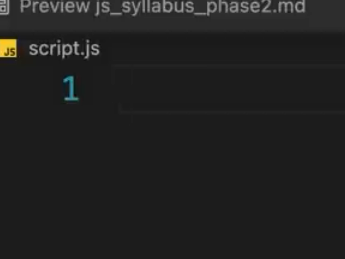
\includegraphics[width=\textwidth]{image.png}
\caption{image 1 is screenshot}
\end{subfigure}
\hfill
\begin{subfigure}[b]{0.25\textwidth}
\centering

\includegraphics[width=\textwidth]{image2.png}
\caption{image 2 of screenshot}
\end{subfigure}
\hfill
\begin{subfigure}[b]{0.25\textwidth}
\centering

\includegraphics[width=\textwidth]{image3.png}
\caption{image 3 as screenshot}
\end{subfigure}
\hfill
\caption{Screenshot images are placed side by side}
\end{figure}
\end{document}